%%%%%%%%%%%%%%%%%%%%%%%%%%%%%%%%% Main Part %%%%%%%%%%%%%%%%%%%%%%%%%%%%%%%%%%

\chapter{Theoretical Background}
\label{chap:background}

\section{Sample Section}

\subsection{Citations and Footnotes}

This is a reference to a paper \citep{Pernul1994}. You can also make a reference to multiple papers \citep{Pernul1994, pernul2009datenbanken}. References are held in the file \textit{References.bib}. References can be managed, e.g., with Mendeley\protect{\footnote{\url{https://www.mendeley.com}}} or JabRef\protect{\footnote{\url{https://www.jabref.org/}}}. If you want to quote something, dont't worry about quotation marks but use 
\textbf{\textbackslash say,} e.g., \say{This is a quote.} \par\smallskip

\subsection{Usage of Abbrevations}

The automatic creation of the list of abbreviations is also very useful. Abbreviations can be defined in main.tex. The abbreviation, e.g. \ac{SaaS}, is defined to appear in the list of abbreviations the first time it is used. Please use an abbreviation consistently once it has been introduced.
Not every use of the same abbreviation needs to be hyperlinked using the \verb+\ac{}+ command. But if there are many pages between the use of an abbreviation hyperlinking can be helpful for the reader.


\subsection{Lists}
There are two forms of lists in Latex, ordered lists (\textbf{enumerate}):
\begin{enumerate}
    \item Point 1
    \item Point 2
    \item Point 3
\end{enumerate}

and bulleted lists (\textbf{itemize}):

\begin{itemize}
    \item Point 1
    \item Point 2
    \item Point 3
\end{itemize}


\subsection{Tables}
\label{sec:tables}

In this section, you find a sample table. Labels of tables are - in contrast to figures - always on top of them.

\begin{table} [h]
\centering
\caption{Sample Table Caption.}
\label{tab:feedback}
\begin{tabular}{lccc}
\toprule
\textbf{Condition} & \textbf{Mean} & \textbf{Median} & \textbf{Standard deviation} \\
\midrule
Value 1 & 4.40 & 5 & 0.75 \\
Value 2 & 4.35 & 4 & 0.72 \\
Value 3 & 4.10 & 4 & 0.78 \\
Value 4 & 4.23 & 4 & 0.72 \\
Value 5 & 4.14 & 4 & 0.79 \\
\bottomrule
\end{tabular}
\end{table}

\subsection{Figures}
\label{sec:figures}

You can adjust the size of your figures according to the textwidth. Figure~\ref{fig:Fig1} one has the full textwidth, Figure~\ref{fig:Fig2} 30\% of it.

\begin{figure} [!htb]
  \centering
  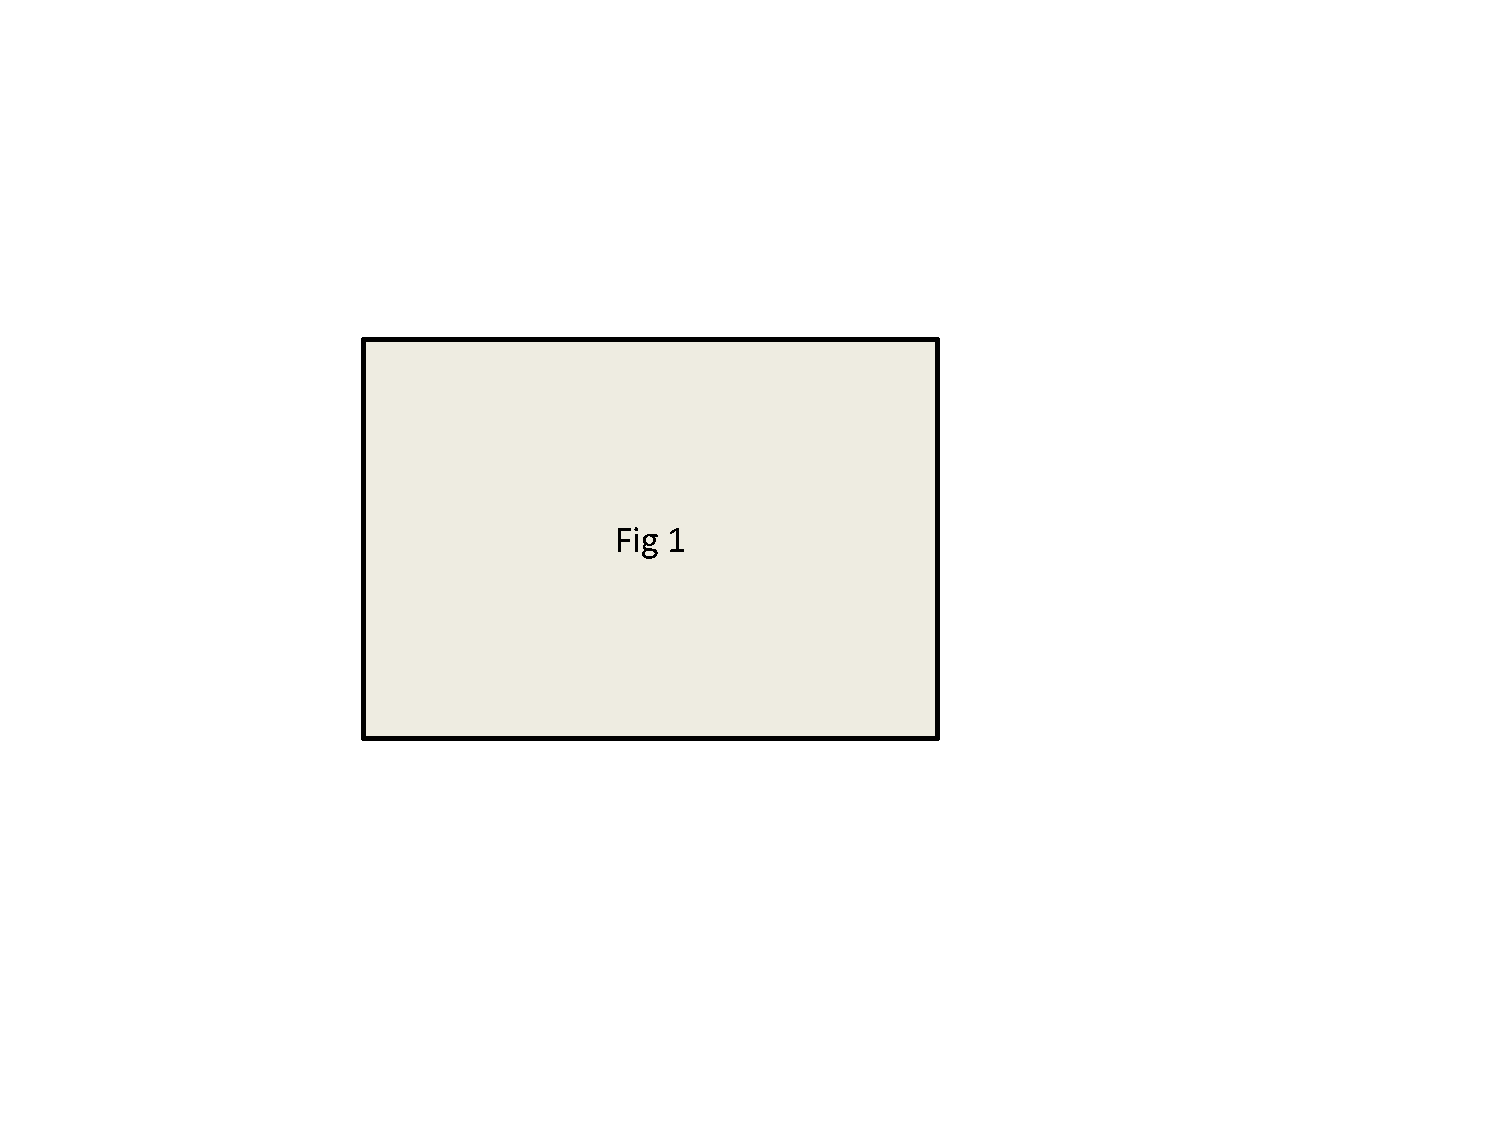
\includegraphics[width=\textwidth]{Fig1.pdf}
  \caption{Sample Figure.}
  \label{fig:Fig1}
\end{figure}


\begin{figure} [!htb]
  \centering
  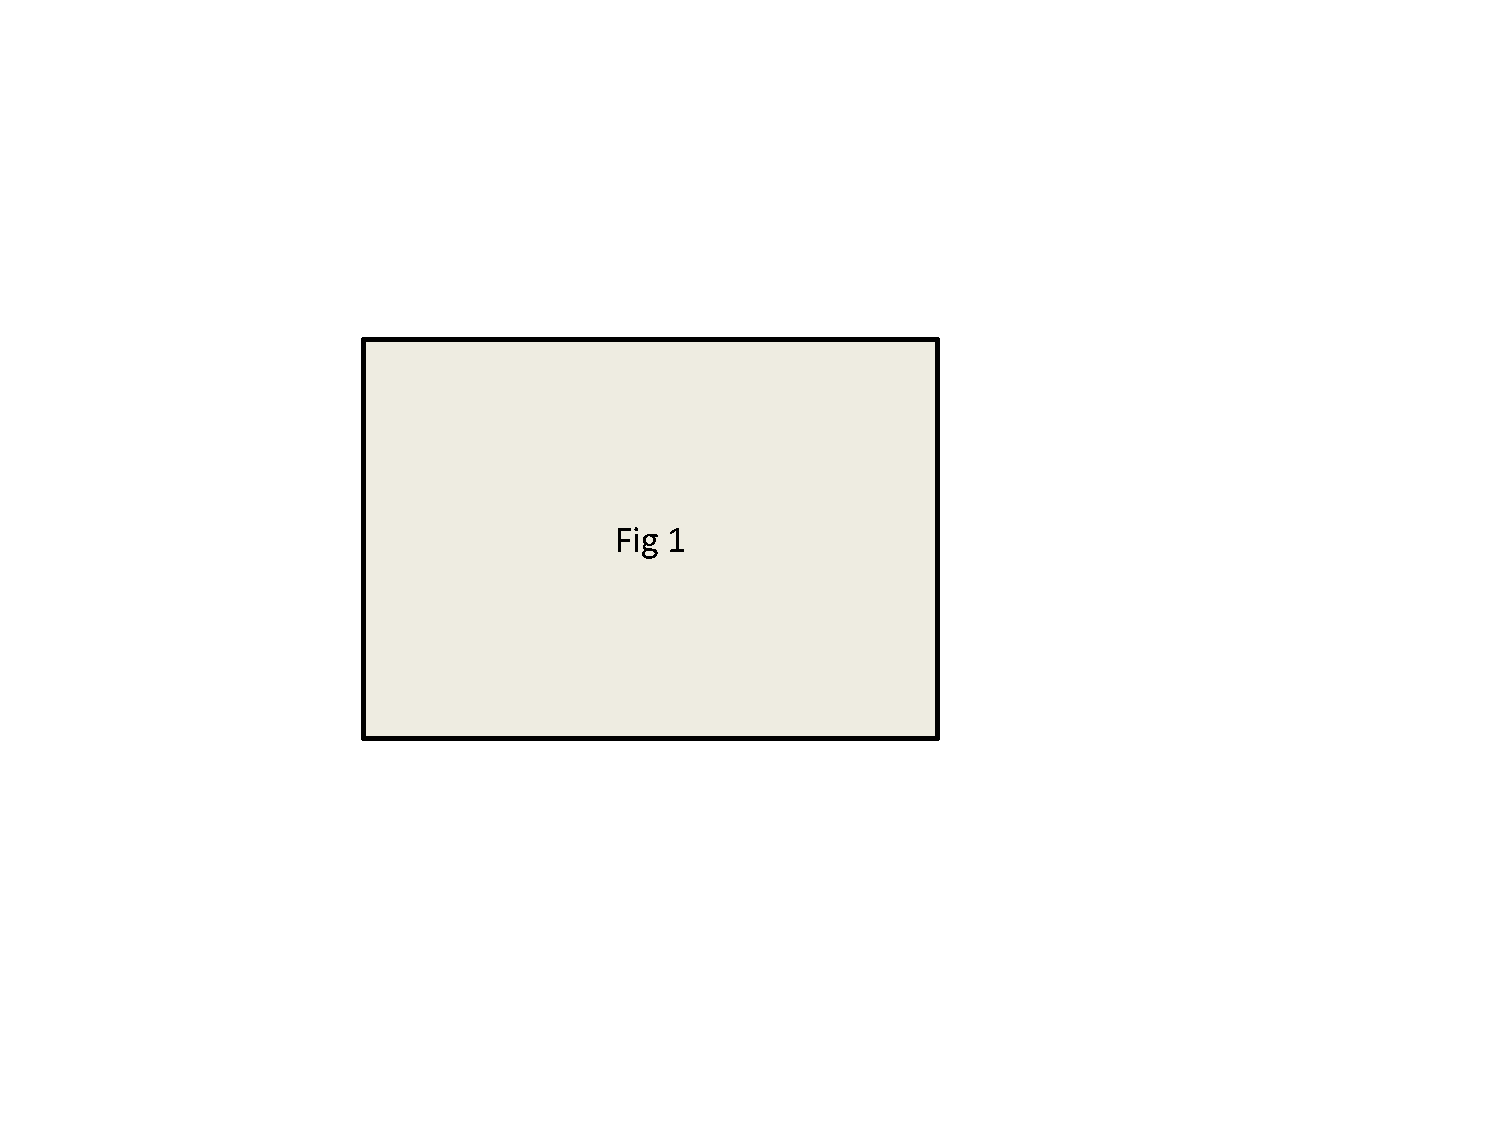
\includegraphics[width=0.3\textwidth]{Fig1.pdf}
 \caption{Sample Smaller Figure.}
  \label{fig:Fig2}
\end{figure}


\subsection{References}

The following sentence demonstrates the usage of references. In Subsection~\ref{sec:figures}) we explained how to use figures in \LaTeX, e.g., Figure~\ref{fig:Fig1}. Don't forget to mention every table, figure or listing you use at least once in your text.

\subsection{Usage of Listings}

\lstset{language=JAVA, breaklines=true, tabsize=2}
\lstinputlisting[caption=HelloWorld,
label=lst:HelloWorld]{listings/HelloWorld.java}



\begin{landscape}

Page in landscape format, e.g., for larger figures or tables; footer remains in portrait format.
\end{landscape}




%%%%%%%%%%%%%%%%%%%%%%%%%%%%%%%%%%%%%%%%%%%%%%%%%%%%%%%%%%%%%%%%%%%%%%%%%%%%%%
